\documentclass{beamer}
\usepackage[russian]{babel}
\usetheme{metropolis}

\usepackage{amsthm}
\setbeamertemplate{theorems}[numbered]

\setbeamercolor{block title}{use=structure,fg=white,bg=gray!75!black}
\setbeamercolor{block body}{use=structure,fg=black,bg=gray!20!white}

\usepackage[T2A]{fontenc}
\usepackage[utf8]{inputenc}

\usepackage{hyphenat}
\usepackage{amsmath}
\usepackage{graphicx}

\AtBeginEnvironment{proof}{\renewcommand{\qedsymbol}{}}{}{}

\title{
Микроэкономика-I
}
\author{
Павел Андреянов, PhD
}

\begin{document}

\maketitle

\begin{frame}{План лекции}

\begin{itemize}
  \item Часть 1. Сложение спроса и предложения. Репрезентативный агент. Сложение эластичностей. Частичное равновесие, PS, CS.
  \item Часть 2. Налоги на потребителя и производителя. DWL. Пол и потолок цены.  Экстерналии
\end{itemize}

Осторожно, я буду иногда путать между собой $x$ и $Q$.
\end{frame}

\section{Сложение спросов}

\begin{frame}{Сложение предложений}

Весь модуль мы работали, для простоты, с 1 потребителем и выводили его спрос. Нас, конечно, будет интересовать 

\begin{itemize}
  \item либо суммарный спрос небольшого количества разных потребителей
  \item либо суммарный спрос большого количества одинаковых потребителей
  \item теоретически, также суммарный спрос большого количества разных потребителей
\end{itemize}

Как происходит суммирование?

\end{frame}

\begin{frame}{Сложение спросов}
В координатах $x,p$ (помним, что у экономистов цена всегда по вертикали), спросы \alert{складываются горизонтально}
    \begin{center}
     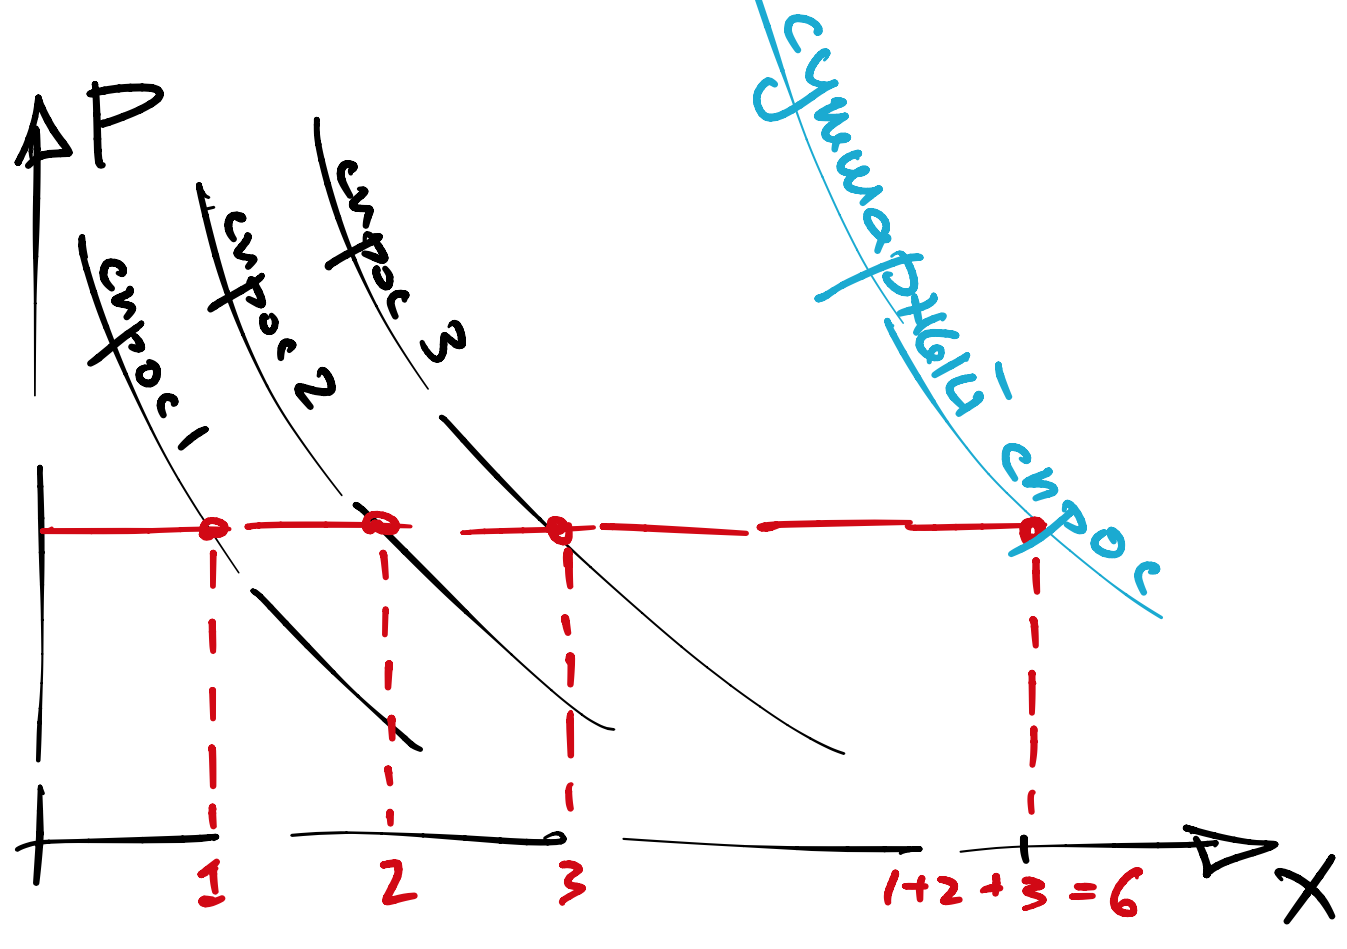
\includegraphics[width=.8\textwidth]{sumdemand}
     \end{center}
\end{frame}

\begin{frame}{Сложение спросов}
Рассмотрим аналитический пример (бюджеты обозначим $I_1, I_2, I_3$, а цены товаров у всех одинаковые: $p,q$)
\begin{itemize}
  \item $U_1 = 2 \log x + 3 \log y$
  \item $U_2 = \log x + 4\log y$
  \item $U_3 = 3\log x + 2\log y$
\end{itemize}
Просуммируем отдельно спросы на товары $x, y$:
$$ x^{sum} = \frac{1}{p}(\frac{2}{5}I_1 + \frac{1}{5}I_2 +\frac{3}{5}I_3), \quad y^{sum} = \frac{1}{q}(\frac{3}{5}I_1 + \frac{4}{5}I_2 +\frac{2}{5}I_3)$$
To есть, сложение Кобб-Дугласов приводит к спросу, который сам чем-то похож на Кобб-Дугласа
\end{frame}

\section{Продвинутое сложение спросов}

\begin{frame}{Сложение спроса}
Рассмотрим экзотический пример, пусть бюджеты распределены, например, равномерно на отрезке $[0,1]$ (тогда сумма превращается в матожидание), а полезность у всех
$$U = 2 \log x + 3 \log y$$
Просуммируем спросы на товар $x$:
$$ x^{sum} = \mathbb{E} \frac{1}{p} \frac{2}{3} I = \frac{1}{p} \frac{2}{3} \mathbb{E} I = \frac{1}{p} \frac{2}{3}\frac{1}{2} = \frac{1}{3p}$$
Потому что матожидание (значок $\mathbb{E}$) линейно
\end{frame}

\begin{frame}{Сложение спросов}
Рассмотрим более экзотический пример, пусть бюджеты равны 1, а параметр $\alpha$ распределен равномерно на отрезке $[0,b]$ (матожидание $\mathbb{E} \alpha = b/2$), а полезность у всех одна и та же
$$U = \alpha \log x + (1-\alpha) \log y$$
Просуммируем спросы на товар $x$:
$$ x^{sum} = \mathbb{E} \frac{1}{p} \alpha = \frac{1}{p} \mathbb{E} \alpha = \frac{1}{p} \frac{b}{2} = \frac{b}{2p}$$
Потому что матожидание линейно
\end{frame}

\begin{frame}{Сложение спросов}
К чему все эти примеры? Вы можете смотреть на кривую спроса и думать про нее как про
\begin{itemize}
  \item спрос одного единственного агента
  \item суммарный спрос большого кол-ва одинаковых агентов
  \item суммарный спрос большого кол-ва разных агентов
\end{itemize}
В частности, вы можете думать про параметры $\alpha, I$ как \alert{арифметические средние} значения веса и бюджета (распределенные независимо) в большой популяции агентов с полезностью Кобб-Дугласа.
\end{frame}

\begin{frame}{Сложение спросов}
Действительно, представим произвольно много агентов. 

Скажем, что агент $i$ обладает весом $\alpha_i$ и бюджетом $I_i$, а масса самих агентов нормирована к единичке. Тогда
$$ \mathbb{E}(x_i) = \mathbb{E} (\frac{\alpha_i I_i}{p}) = \frac{1}{p} \mathbb{E}(\alpha_i I_i) = \frac{1}{p} \mathbb{E}(\alpha_i) \mathbb{E}(I_i)$$
С точки зрения наблюдателя это невозможно отличить от ситуации, в которой есть только один (нулевой) агент с параметрами $\alpha_0 =\mathbb{E}(\alpha_i)$ и $I_0 =\mathbb{E}(I_i)$.

Такой агент называется \alert{репрезентативным}.

\end{frame}

\section{Сложение не КД}

\begin{frame}{Сложение не КД}

Спросы могут складываться более или менее удачно. 

У всех полезностей, обладающих свойством \alert{гомотетичности} (кривые безразличия подобны друг другу и расширяются от центра координат) суммарный спрос одинаковых агентов с разными бюджетами ведет себя так же как и спрос одного единственного (репрезентативного) агента с суммарным бюджетом. 

Другими словами, спрос \alert{шкалируется по доходу}.

\end{frame}

\begin{frame}{Сложение не КД}

Большая часть полезностей гомотетичные:
\begin{itemize}
  \item кобб дуглас
  \item леонтьев
  \item линейная
  \item ces
\end{itemize}
и спрос в них шкалируется по доходу.

Важным исключением является квазилинейная полезность, спрос в ней шкалируется не по доходу а по числу агентов.

\end{frame}

\section{Сложение совсем разных спросов}

\begin{frame}{Сложение совсем разных спросов}

До сих пор я складывал спросы одной природы: кд с кд, леонтьев с леонтьев, итд. Поэтому ответ получался простой и предсказуемый. В частности, поскольку все простые спросы линейны по бюджету, суммирование одинаковых агентов с разными бюджетами сводилось к суммированию бюджетов.

Что будет если мы сложим КД с Леонтьевым?
\end{frame}

\begin{frame}{Сложение совсем разных спросов}
Возьмем две такие полезности
$$ U_1 = \alpha \log x + \beta \log y, \quad U_2 = \min(\frac{x}{a},\frac{y}{b})$$
И сложим спросы...
\begin{gather*}x^{sum} =(\frac{\alpha}{\alpha+\beta} + \frac{ap}{ap+bq})\frac{I}{p},\\ y^{sum} =(\frac{\beta}{\alpha+\beta} + \frac{bq}{ap+bq})\frac{I}{p}\end{gather*}
... ничего особо интересного.

Разве что интересно как преобразуются эластичности.
\end{frame}

\section{Сложение эластичностей}

\begin{frame}{Сложение эластичностей}
Поскольку суммарный спрос это сумма спросов,
$$ \frac{\partial x^{sum}}{\partial p} = \sum \frac{\partial x}{\partial p}$$
Но нам то надо
$$ \varepsilon_{x,p}^{sum} = \frac{\partial x^{sum}}{\partial p} \frac{p}{x^{sum}}= \sum_k \frac{\partial x^k}{\partial p}\frac{p}{x^{sum}} = ?$$
тут $k$ это индекс агента. Попробуем у доски?
\end{frame}

\begin{frame}{Сложение эластичностей}
Напомним
$$ \varepsilon_{x,p}^{sum} = \frac{\partial x^{sum}}{\partial p} \frac{p}{x^{sum}}= \sum_k \frac{\partial x^k}{\partial p}\frac{p}{x^{sum}} = ...$$
далее
$$ ... = \sum_k (\frac{\partial x^k}{\partial p}\frac{p}{x^k})(\frac{x^k}{p}\frac{p}{x^{sum}}) = \sum_k (\varepsilon^k_{x,p} \cdot \frac{x^k}{x^{sum}})$$
тут $k$ это индекс агента.

То есть, \alert{эластичность суммарного спроса это средневзвешенная эластичность индивидуальных спросов}. 

Причем веса пропорциональны самим спросам в этой точке.
\end{frame}

\begin{frame}{Сложение эластичностей}
Это знание может сэкономить вам время на контрольной.

Решим какой нибудь пример (скажем, кд + леонтьев) у доски
\end{frame}

\section{Сложение предложений}

\begin{frame}{Сложение предложений}
В координатах $x,p$ (помним, что у экономистов цена всегда по вертикали), предложения \alert{складываются тоже горизонтально}
    \begin{center}
     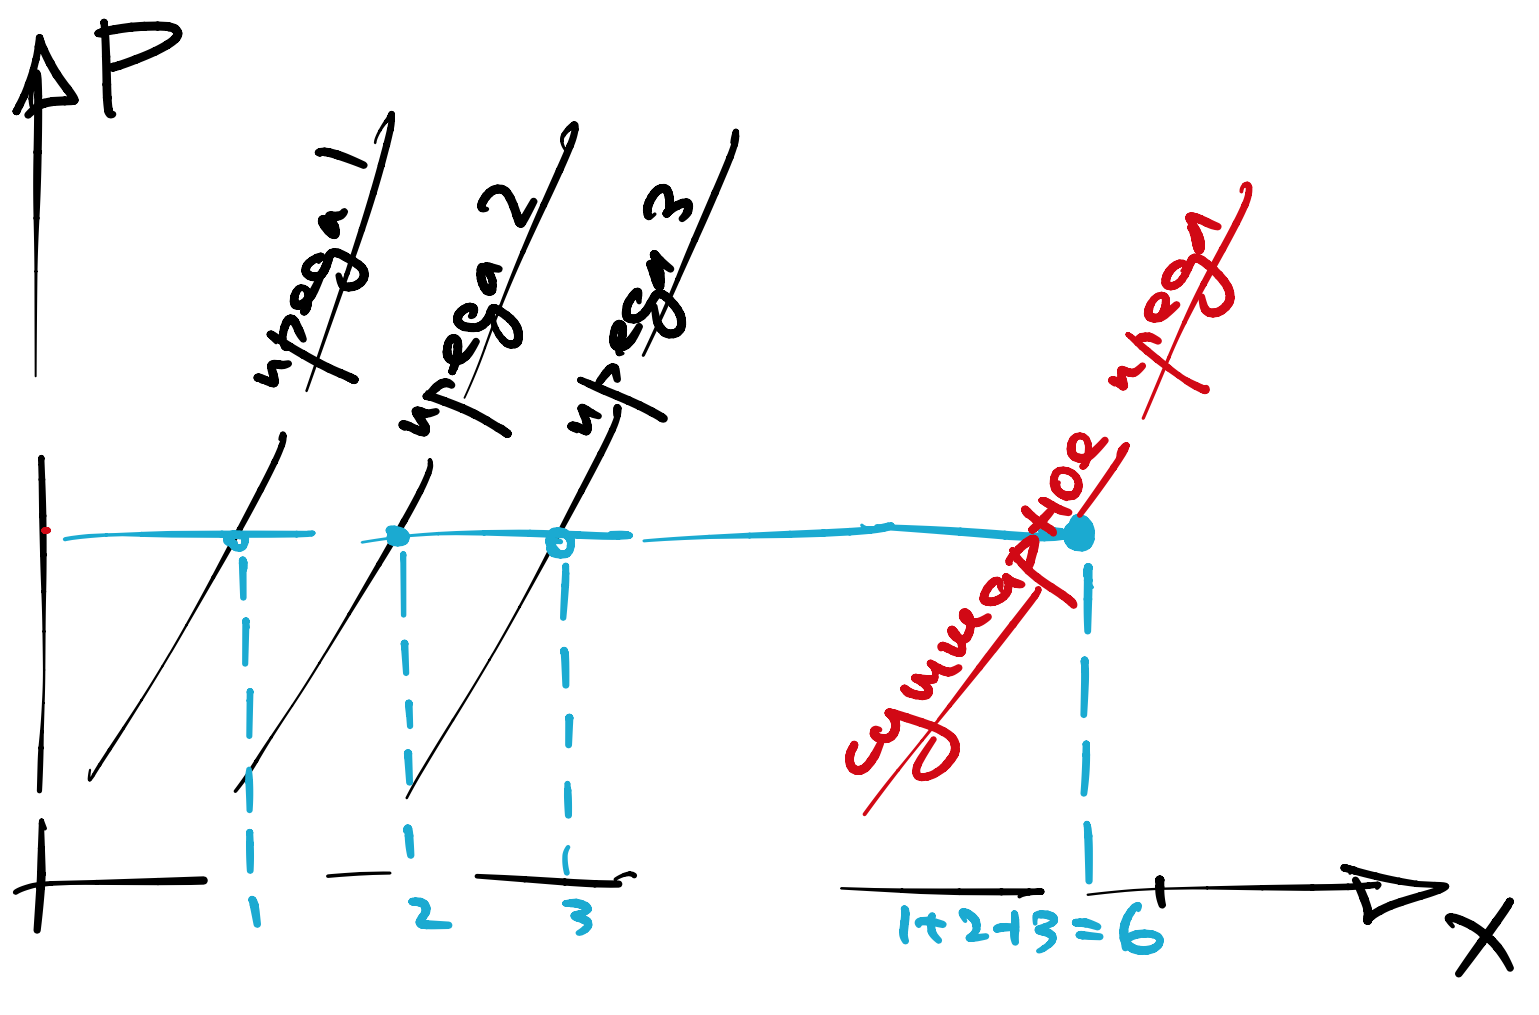
\includegraphics[width=.8\textwidth]{sumsupply}
     \end{center}
\end{frame}

\begin{frame}{Сложение предложений}

Задачу фирмы можно сформулировать по-разному.
\begin{itemize}
  \item Можно задать функции издержек каждой фирмы
  \item Можно задать производственную функцию каждой фирмы
  \item Можно задать технологическое множество каждой фирмы
\end{itemize}
Первый способ для нас самый естественный

\alert{Внимание:} Чтобы не лезть в греческий алфавит,\\ \alert{я буду предложение товара $x$ обозначать заглавной буквой $X$}. Спрос будет  обозначаться, как и сам товар, прописной $x$.

\end{frame}

\begin{frame}{Сложение предложений}
\begin{itemize}
  \item $TC^1(X,Y) = X^2 + X + Y^2$
  \item $TC^2(X,Y) = X^2/2 + X + Y^2$
  \item $TC^3(X,Y) = X^2 + Y^2$
\end{itemize}
Пусть есть три фирмы с издержками (цены товаров равны $p,q$). Каждая из них производит функцию предложения (первого) товара $x$, по чистому совпадению не зависящая от цены (второго) товара $y$
$$ X^{sum} = \frac{p-1}{2} + (p-1) + \frac{p}{2} = 2p - \frac{3}{2}$$
Суммарное предложения (второго) товара $y$ также чудом не зависит от цены первого
$$ Y^{sum} = \frac{3}{2} q $$ 
\end{frame}

\begin{frame}{Сложение предложений}
Теперь я хочу сделать кое что странное...
\begin{itemize}
  \item $TC^1(X,Y) = X^2 + X + Y^2$
  \item $TC^2(X,Y) = X^2/2 + X + Y^2$
  \item $TC^3(X,Y) = X^2 + Y^2$
\end{itemize}
Давайте посчитаем суммарную функцию издержек...
$$ TC^{sum} \neq \frac{5}{2} X^2 + 2X + 3 Y^2$$
... только по правилам сложения функций издержек.
$$ (X_1^2 + X_1) + (X_2^2/2 + X_2) + X^2_3 \to \min, \quad X_1 + X_2 + X_3 = X$$
\end{frame}

\begin{frame}{Сложение предложений}
$$ (X_1^2 + X_1) + (X_2^2/2 + X_2) + X^2_3 \to \min, \quad X_1 + X_2 + X_3 = X$$
Выпишем фоки
\begin{itemize}
  \item $MC^1 = 2 X_1 + 1 = \lambda$
  \item $MC^2 = X_2 + 1 = \lambda$
  \item $MC^3 = 2 X_3 = \lambda$
  \item $X_1 + X_2 + X_3 = X$
\end{itemize}
В вольфрамальфа я могу заказать решение в одну строку \text{solve 2*x1+1 == l, x2+1==l, 2*x3==l, x1+x2+x3==x for l,x1,x2,x3}

\end{frame}

\begin{frame}{Сложение предложений}
Получим решение
$$X^{\ast}_1 = \frac{2X - 1}{8}, \quad X^{\ast}_2 = \frac{2X - 1}{4}, \quad X^{\ast}_3 = \frac{2X + 3}{8}$$
И теперь, с божьей помощью, выпишем (производную, чтобы не тратить время) от суммарной функции издержек
\begin{gather*}MC^{sum}(X) = MC^1(X^{\ast}_1)\frac{\partial X^{\ast}_1}{\partial X} + MC^2(X^{\ast}_2)\frac{\partial X^{\ast}_2}{\partial X} + MC^3(X^{\ast}_3)\frac{\partial X^{\ast}_3}{\partial X} = \\ = (\frac{2X - 1}{4} + 1)\frac{1}{4} + (\frac{2X-1}{4} + 1)\frac{1}{2} + (\frac{2X+3}{4})\frac{1}{4} = \frac{X}{2} + \frac{3}{4}\end{gather*}
\end{frame}

\begin{frame}{Сложение предложений}
И теперь, с божьей помощью, выпишем (производную, чтобы не тратить время) от суммарной функции издержек
\begin{gather*}MC^{sum}(X) = \frac{X}{2} + \frac{3}{4}\end{gather*}
И функция спроса объединенного завода, соответственно, равна $$MC^{sum}(X) = p \quad \Rightarrow \quad X = 2p - \frac{3}{2}$$
... хм, где-то я уже это видел
\end{frame}

\begin{frame}{Сложение предложений}
Удивительным образом, спрос объединенного завода оказался равен суммарному спросу (сумме независимо посчитанных спросов каждого из трех заводов).
$$X^{sum} = 2p - \frac{3}{2}.$$

Совпадение?
\end{frame}

\begin{frame}{Сложение предложений}
Совпадение? Конечно нет!

Дело в том, что система
\begin{itemize}
  \item $MC^1 = 2 X_1 + 1 = p$
  \item $MC^2 = X_2 + 1 = p$
  \item $MC^3 = 2 X_3 = p$
  \item $X_1 + X_2 + X_3 = X$
\end{itemize}
описывает одновременно как сложение индивидуальных спросов так и оптимальное распределение мощностей между тремя заводами, если заменить множитель Лагранжа $\lambda$ на $p$.
\end{frame}

\begin{frame}{Сложение предложений}
Другими словами, на конкурентном рынке нет смысла объединять заводы, они все равно будут поставлять продукцию по правилу $P=MC$. Потому что конкурентный рынок заставляет заводы работать эффективно.

А когда имеет смысл?
\end{frame}

\begin{frame}{Сложение предложений}
А когда имеет смысл? 

Когда рынок не конкурентный, например фирма планирует стать монополистом и контролировать цену. Тогда, для применения закона обратной эластичности ей потребуется сосчитать тот самый злосчастный $MC^{sum}(X)$.
\end{frame}

\begin{frame}{Сложение предложений}

А на контрольной, получается, \alert{вы можете посчитать функцию предложения объединенного завода в обход вывода технологии самого этого завода}, что гораааааздо быстрее и проще.

\begin{itemize}
  \item аналогично если вам даны производственные функции
  \item аналогично если вам даны технологические множества 
\end{itemize}

\end{frame}

\section{Частичное равновесие}

\begin{frame}{Частичное равновесие}

\alert{Частичное равновесие} - это равновесие на рынке одного товара (например $x$) такое что суммарный спрос равен суммарному предложению. То есть, это пара $(x^{\ast}, p^{\ast})$ такие что 
$$ x^{\ast} = x^{sum}(p^{\ast}) = X^{sum}(p^{\ast})$$
При цене $p^{\ast}$ у вас нет ни дефицита ни излишков товара.

Все остальные товары (например $y$) и цены этих товаров ($q$) в частичном равновесии игнорируются, или подразумеваются фиксированными на известном уровне.

\end{frame}

\begin{frame}{Частичное равновесие}
В координатах $x,p$ (помним, что у экономистов цена всегда по вертикали), частичное равновесие это просто координаты пересечения суммарного спроса с суммарным предложением
    \begin{center}
     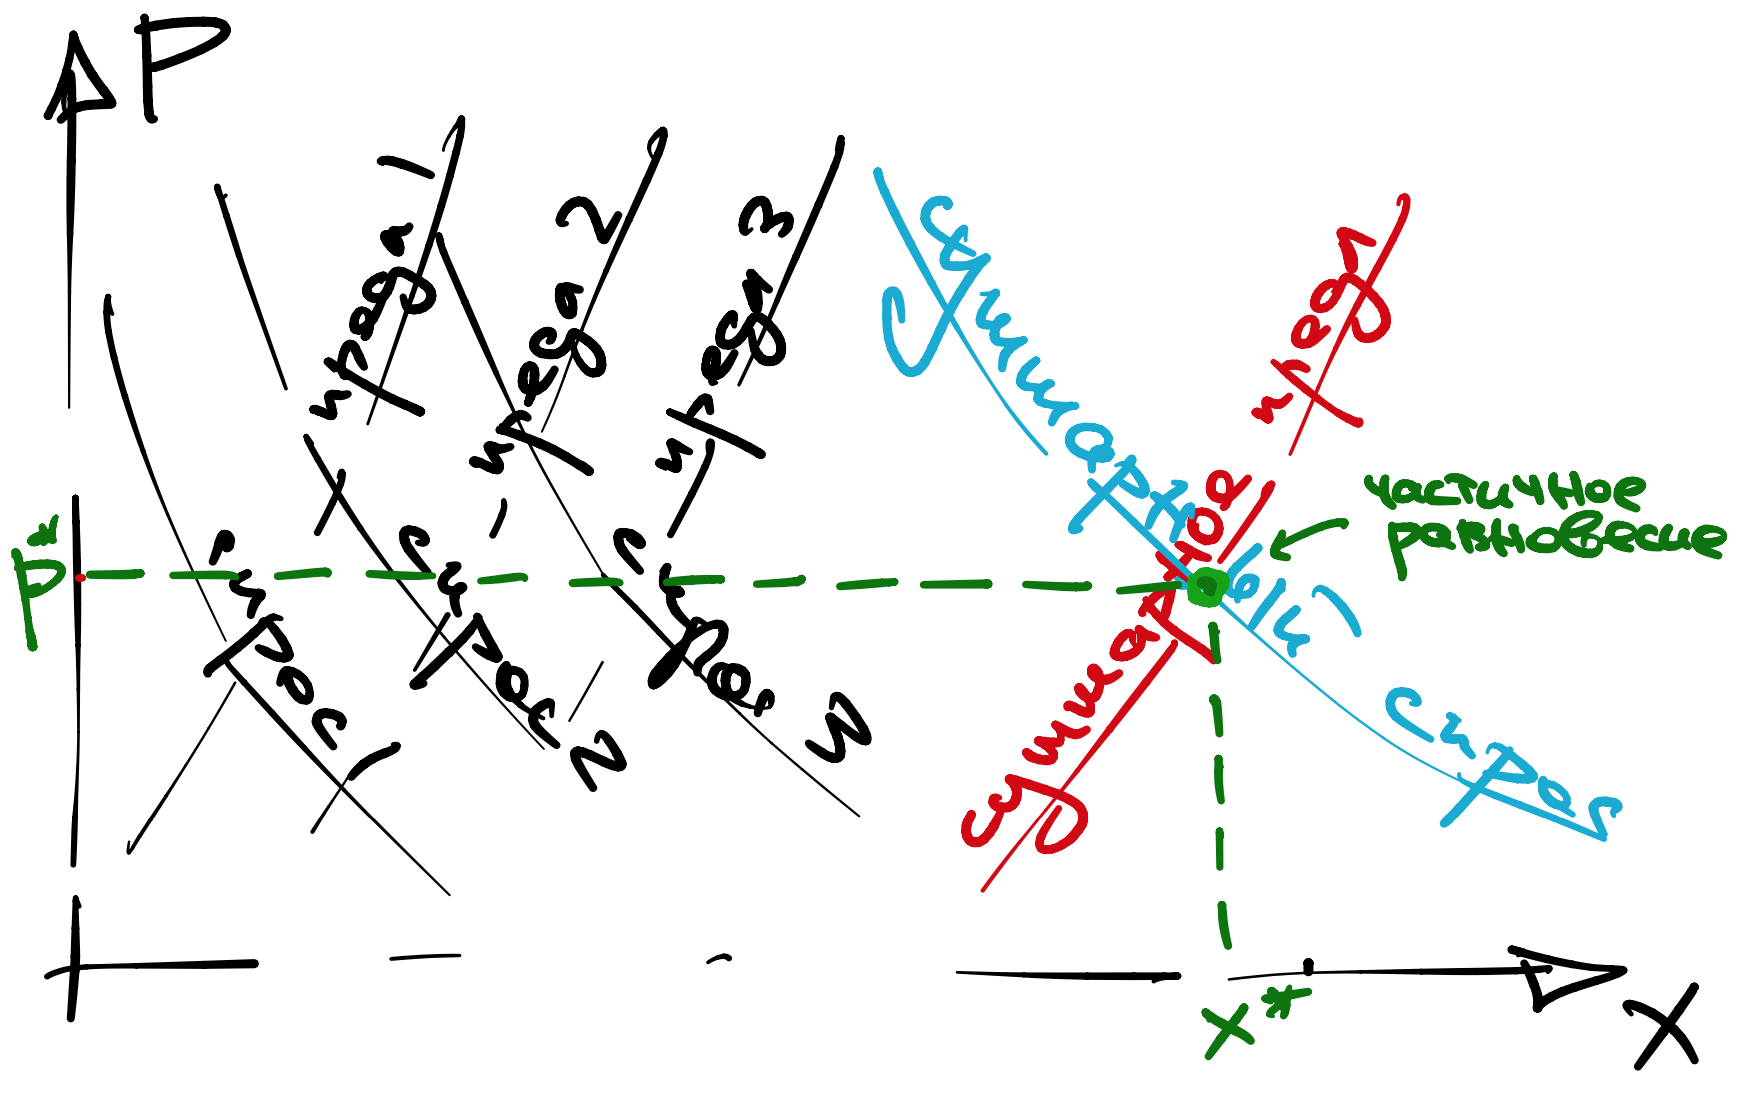
\includegraphics[width=.8\textwidth]{partial}
     \end{center}
\end{frame}

\begin{frame}{Частичное равновесие}
Аналитически, это просто решение системы уравнений
$$\begin{cases}
  x = x^{sum}(p) \\
  x = X^{sum}(p)
\end{cases}$$

Напомню, что заглавная $X^{sum}$ это суммарное предложение, а прописная $x^{sum}$ это суммарный спрос.

\alert{Внимание}: эластичности есть как у спроса так и у предложения. Чтобы различать их между собой \alert{я буду эластичность предложения обозначать заглавной буквой $\mathcal{E}^{sum}$}, а прописную $\varepsilon^{sum}$ оставим, как и раньше, для потребителя.

\end{frame}

\section{PS и CS}

\begin{frame}{Излишек производителя (PS)}
\begin{columns}
\begin{column}{0.45\textwidth}
   \alert{Излишек производителя это} площадь между кривой предложения и равновесной ценой, зажатая между нулем и актуальным (по любым причинам) количеством проданного товара.
   
   \medskip
   
   Формально, $PS = PQ - \int_0^Q MC(x) dx = PQ - TC(Q) + TC(0) = \alert{\text{чистая прибыль} + FC}$
   
   \end{column}
\begin{column}{0.55\textwidth}  %%<--- here
    \begin{center}
     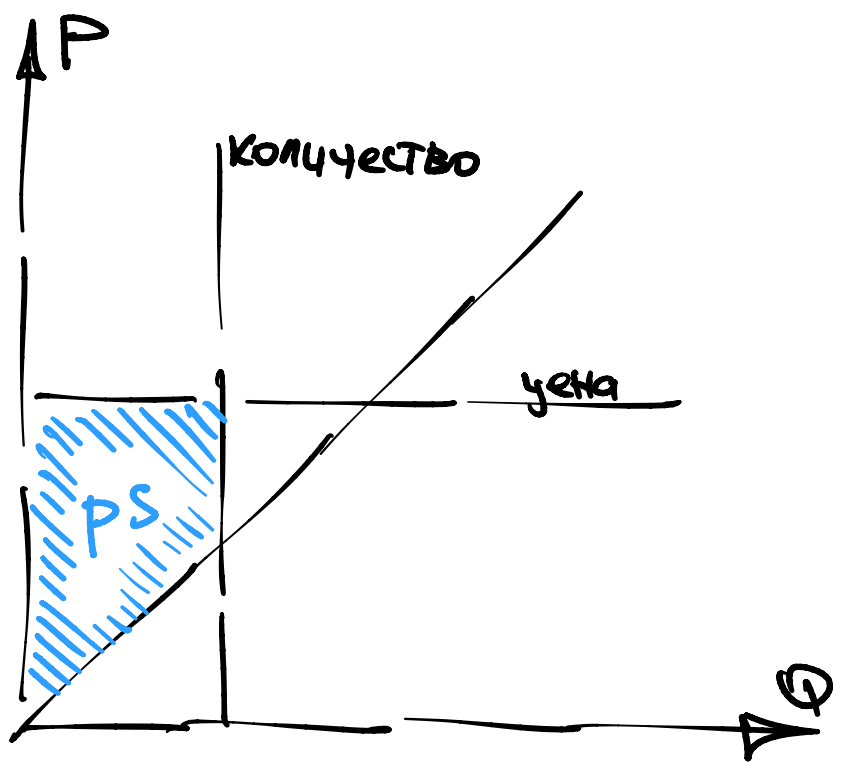
\includegraphics[width=1\textwidth]{PS}
     \end{center}
\end{column}
\end{columns}
\end{frame}

\begin{frame}{Излишек потребителя (CS)}
\begin{columns}
\begin{column}{0.45\textwidth}
   \alert{Излишек потребителя это} площадь между кривой спроса и равновесной ценой, зажатая между нулем и актуальным (по любой причине) количеством проданного товара.
   
   \medskip
   
   В квазилинейной экономике $CS = \int_0^Q MU(x) dx - PQ = U(Q) -  U(0) - PQ = \alert{\text{чистая полезность}}$
   
   
   \end{column}
\begin{column}{0.55\textwidth}  %%<--- here
    \begin{center}
     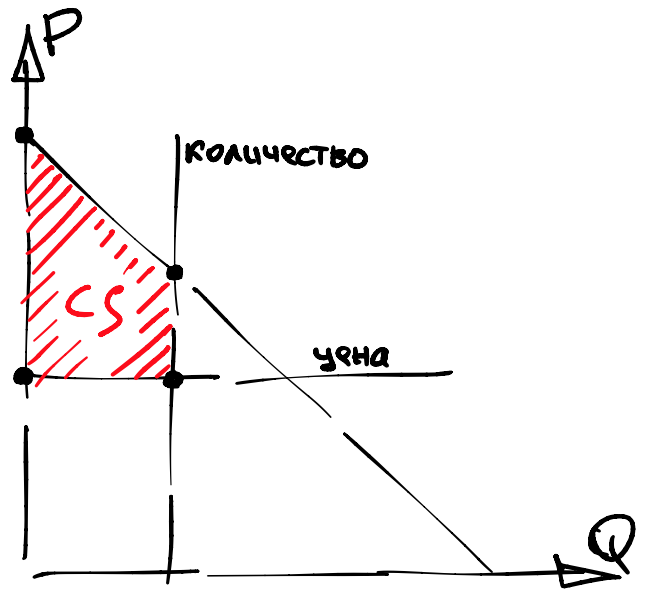
\includegraphics[width=1\textwidth]{CS}
     \end{center}
\end{column}
\end{columns}
\end{frame}

\begin{frame}{Сумма излишков (TS = CS + PS)}
\begin{columns}
\begin{column}{0.45\textwidth}
   Хорошо известно, что сумма излишков потребителя и производителя $TS = CS+PS$ максимизируется, когда количество проданного товара определяется пересечением кривых спроса и предложения.   
   
  \medskip
  
  Все остальные конфигурации рынка могут только повредить TS.
   
   \end{column}
\begin{column}{0.55\textwidth}  %%<--- here
    \begin{center}
     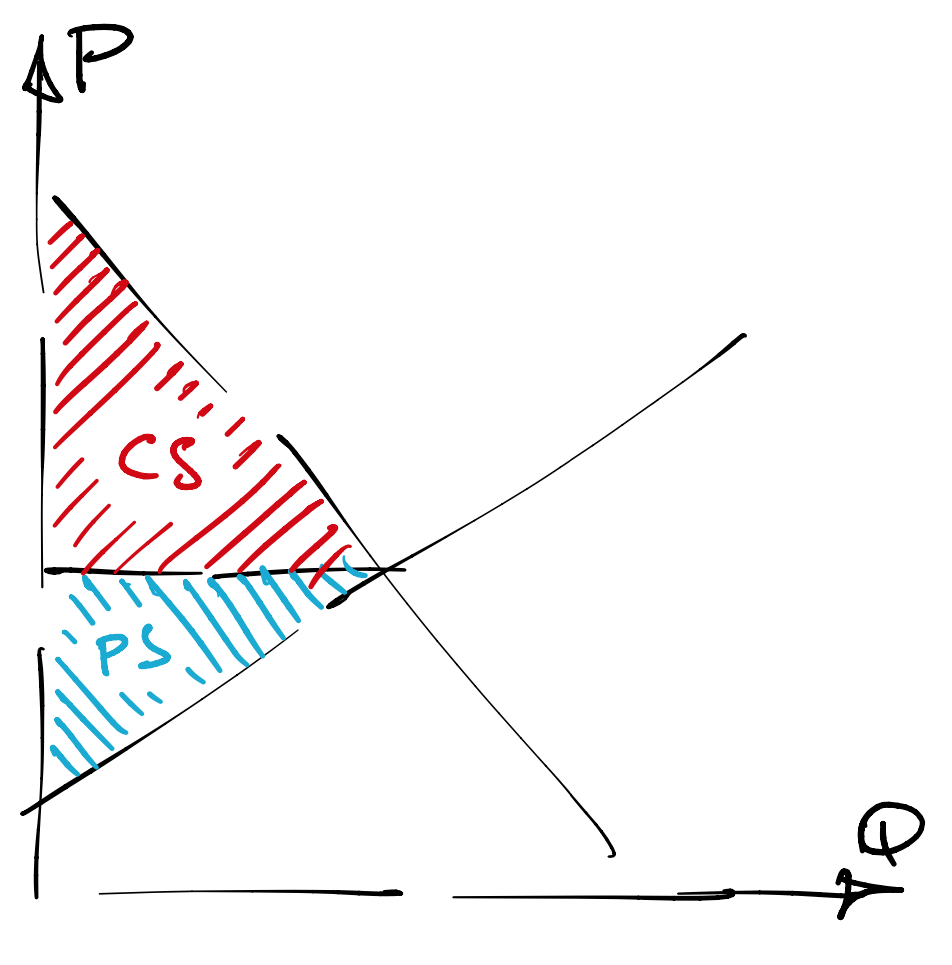
\includegraphics[width=1\textwidth]{CSPS}
     \end{center}
\end{column}
\end{columns}
\end{frame}

\section{Перерыв}

\begin{frame}{Частичное равновесие}

На самом деле, частичным равновесием я называю целый класс задач, в которых могут присутствовать
\begin{itemize}
  \item налоги и субсидии
  \item экстерналии
  \item общественные блага
  \item ...
\end{itemize}
Ключевой момент - это то что рассматривается \alert{рынок одного товара}, а все остальные товары как-бы игнорируются. 

Несмотря на кажущуюся ложность постановки вопроса, в этой модели можно выработать много интересных результатов.
\end{frame}

\begin{frame}{Частичное равновесие}
Например, одним из таких результатов является утверждение о том, что \alert{доли налогового бремени распределяется между потребителями/производителями обратно пропорционально эластичностям спроса/предложения}. 

В англоязычной литературе можно найти более тупую версию того же самого утверждения: <<When supply is more elastic than demand, consumers will bear more of the burden of a tax than producers will.>>

Сегодня мы с вами это все поймем и докажем.
\end{frame}

\section{Налог в частичном равновесии}

\begin{frame}{Частичное равновесие}
В чем суть проблемы?

Есть понятная отрасль, например, молочная продукция (молочка). Это основной источник белка и кальция, поэтому спрос на нее обладает относительно низкой эластичностью.

Поэтому, мы знаем, что государство будет облагать ее налогом, потому что это оптимально с точки зрения правила Рамсея.

Я даже не буду рассматривать паушальный налог, это позапрошлый век (см. оброк - повинность крестьянина платить барину).

\end{frame}

\begin{frame}{Частичное равновесие}

 Может быть, это будет единый для всех товаров НДС, может, он будет дифференциированым, это нас сейчас не волнует. Потому что \alert{мы на рынке одного товара}.

Важным сейчас является то, что налог, вообще говоря, можно применять как к потребителям так и к производителям.

С геометрической точки зрения, это просто сдвиг одной из двух кривых спроса, так как вы подменяете фундаментальные цены $p$ на новые цены с налогом $p + \tau$.

\end{frame}

\begin{frame}{Частичное равновесие}

С геометрической точки зрения, это просто сдвиг одной из двух кривых спроса, так как вы подменяете фундаментальные цены $p$ на новые цены с налогом $p + \tau$.

    \begin{center}
     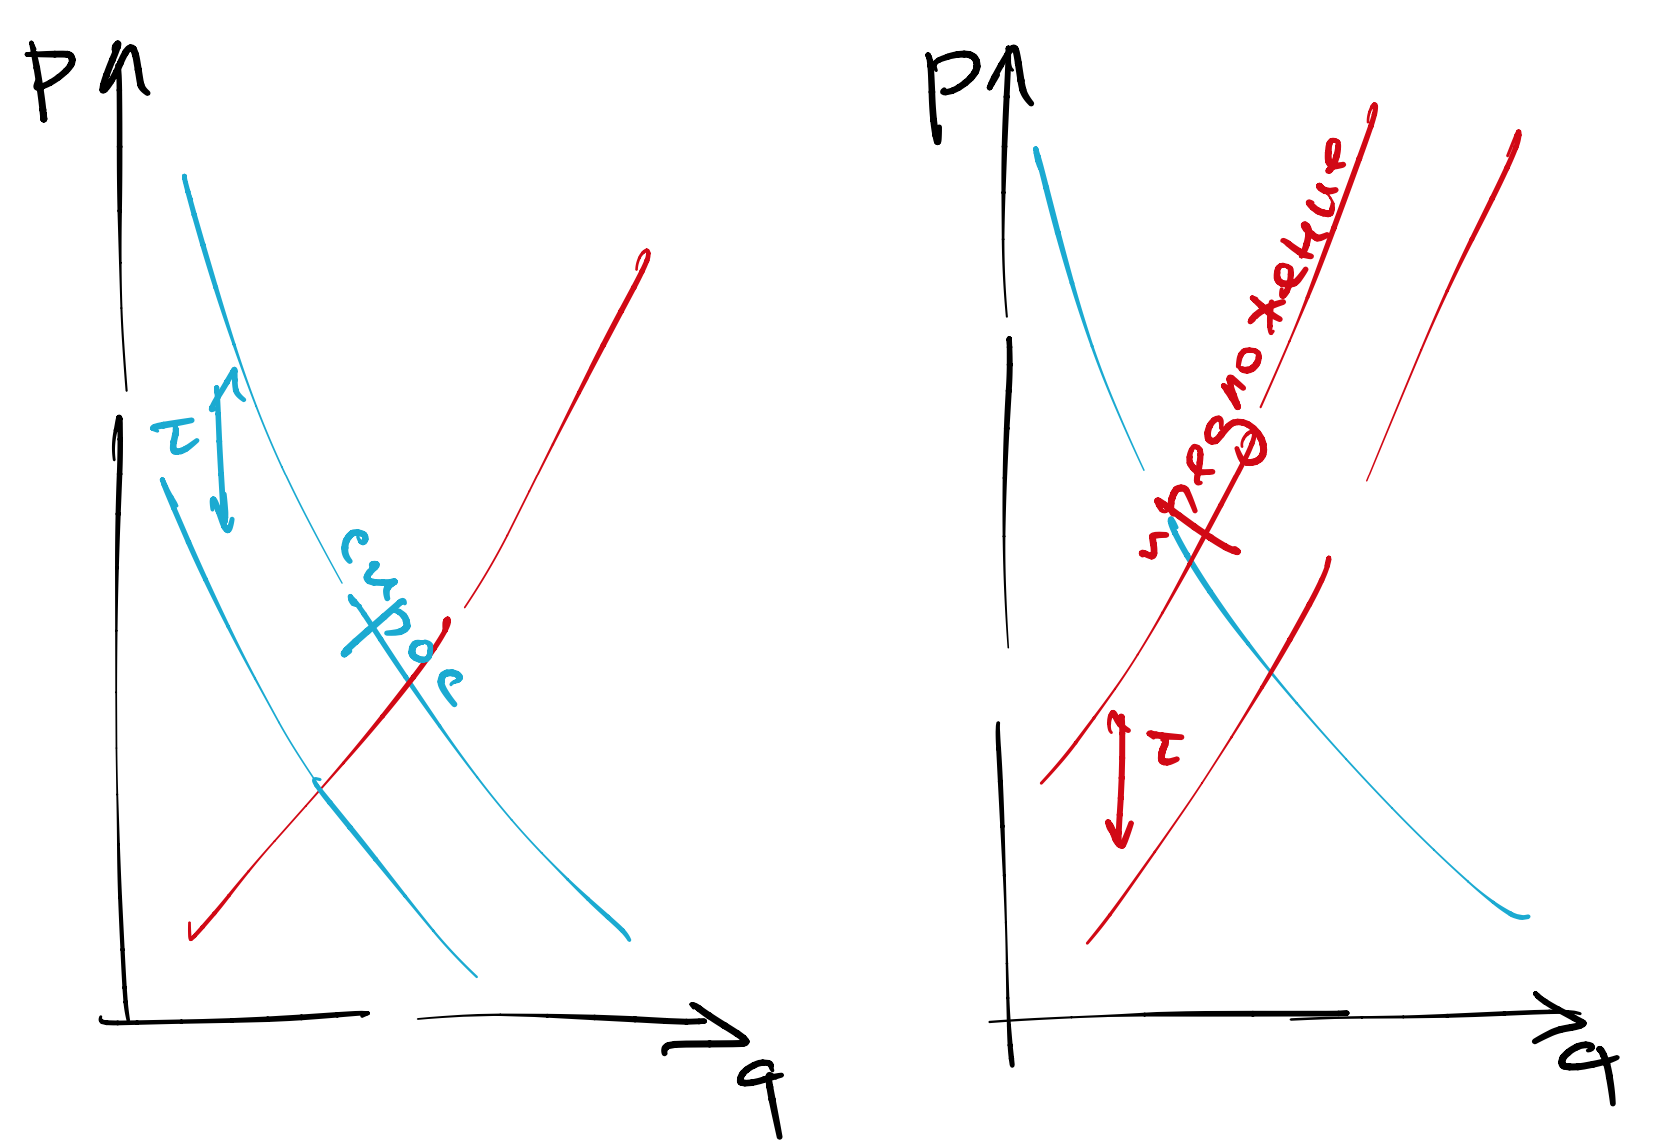
\includegraphics[width=.8\textwidth]{taxes}
     \end{center}
     
Почему так?

\end{frame}

\begin{frame}{Налог на потребителя}

Предположим, что это налог на потребителя, и размера $\tau$.

Если раньше я был готов покупать, скажем, 10 единиц товара по цене $p$ то теперь я готов покупать 10 единиц товара по цене $p-\tau$. Потому что с меня потом возьмут $\tau$.

Подмена аргумента функции спроса с $p$ на $p-\tau$ приводит к съезжанию графика функции спроса вниз (в координатах $x,p$) ровно на $\tau$.

\end{frame}

\begin{frame}{Налог на потребителя}
\begin{columns}
\begin{column}{0.5\textwidth}
   По другому, мы можем сказать что готовность платить за $x$ единиц товара упала, в точности, с $p$ рублей до $p-\tau$ рублей (за штуку). 
   
   \medskip
   
   Как раз, из-за налога $\tau$. 
   
   \medskip
   
   Падение платежеспособности описывается при помощи съезжания графика функции спроса вниз.
\end{column}
\begin{column}{0.5\textwidth}  %%<--- here
    \begin{center}
     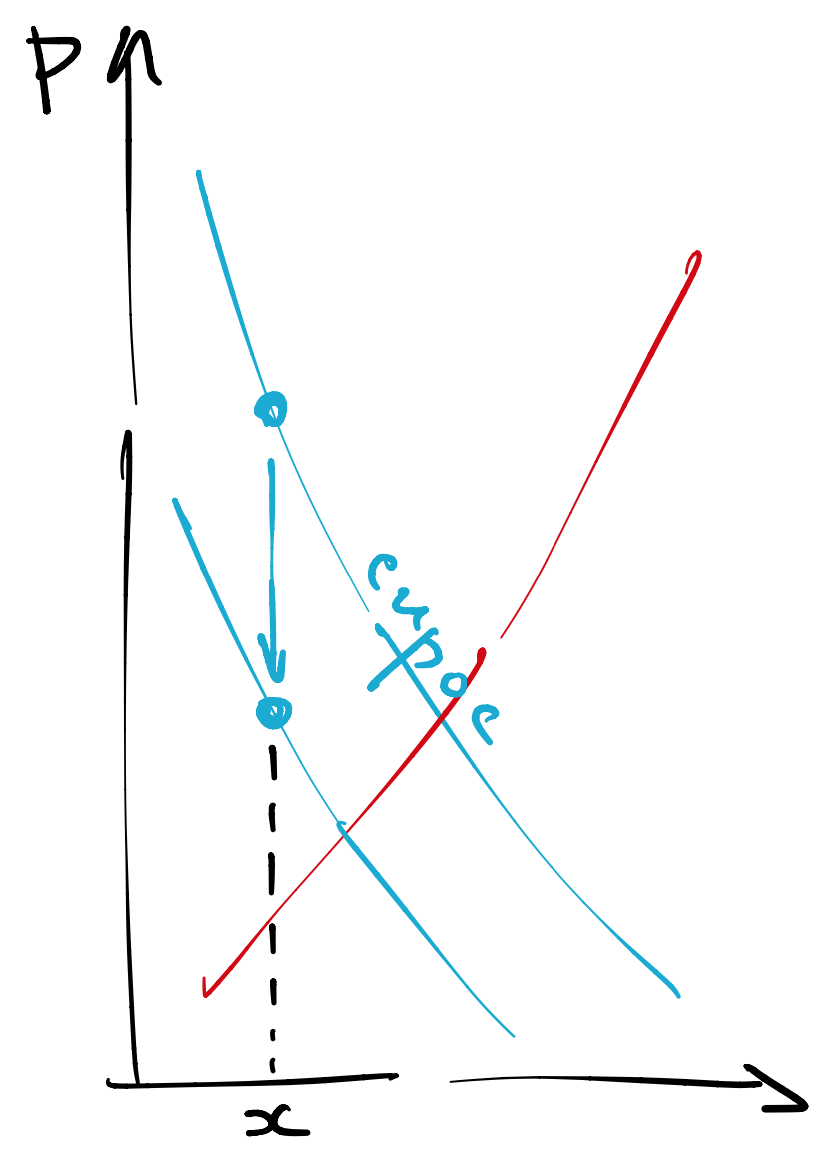
\includegraphics[width=1\textwidth]{constax}
     \end{center}
\end{column}
\end{columns}
\end{frame}

\begin{frame}{Налог на производителя}

Предположим, что это налог на производителя, и размера $\tau$.

Если раньше я был готов производить, скажем, 10 единиц товара по цене $p$ то теперь я готов производить 10 единиц товара по цене $p-\tau$. Потому что с меня потом возьмут $\tau$.

Подмена аргумента функции предложения с $p$ на $p-\tau$ приводит к съезжанию графика функции предложения вниз (в координатах $x,p$) ровно на $\tau$.

\end{frame}

\begin{frame}{Налог на производителя}
\begin{columns}
\begin{column}{0.5\textwidth}
   По другому, мы можем сказать что готовность поставлять $x$ единиц товара упала, в точности, с $p$ рублей до $p-\tau$ рублей (за штуку). 
   
   \medskip
   
   Как раз, из-за налога $\tau$. 
   
   \medskip
   
   Падение платежеспособности описывается при помощи съезжания графика функции предложения вниз.
\end{column}
\begin{column}{0.5\textwidth}  %%<--- here
    \begin{center}
     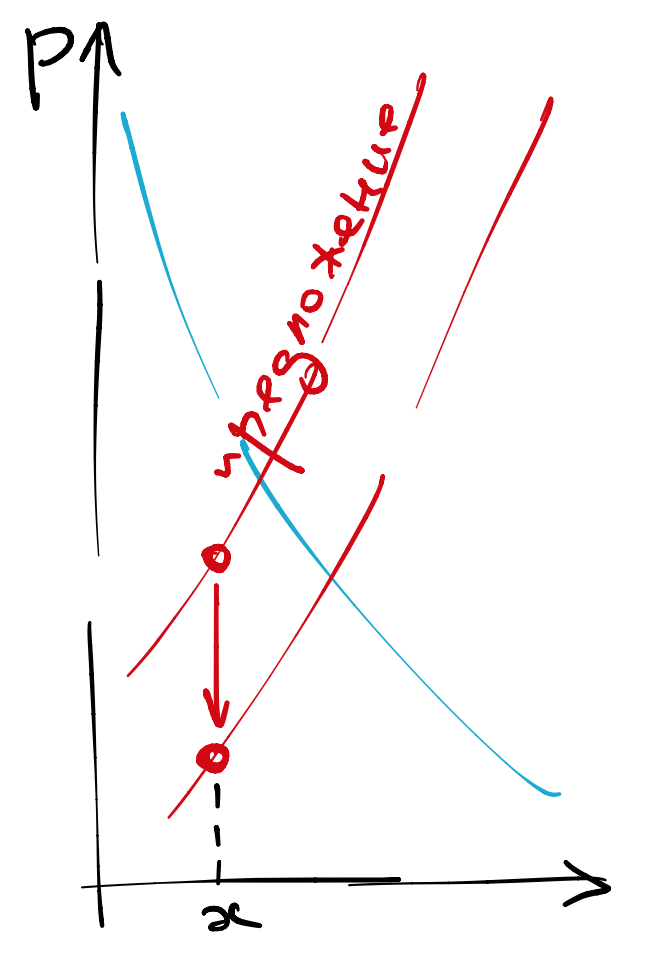
\includegraphics[width=1\textwidth]{prodtax}
     \end{center}
\end{column}
\end{columns}
\end{frame}

\begin{frame}{Налог в ЧР}

Удивительным образом, на определенном уровне абстракции, частичное равновесие вообще не зависит от того, на кого был возложен налог.

\alert{Можно думать про налог в ЧР как расщепление рыночной цены на две: цену потребителя и цену производителя.}

\end{frame}

\begin{frame}{Налог в ЧР}
\begin{columns}
\begin{column}{0.5\textwidth}
   Первая (более высокая) это цена которую воспринимает потребитель.
   
   \medskip
   
   Вторая (более низкая) это цена которую воспринимает производитель.
   
   \medskip
   
   Цены подстраиваются так, что спрос и предложение товара (при соответствующих ценах) совпадают. 
   
   \medskip
   
   Это и есть ЧР.
\end{column}
\begin{column}{0.5\textwidth}  %%<--- here
    \begin{center}
     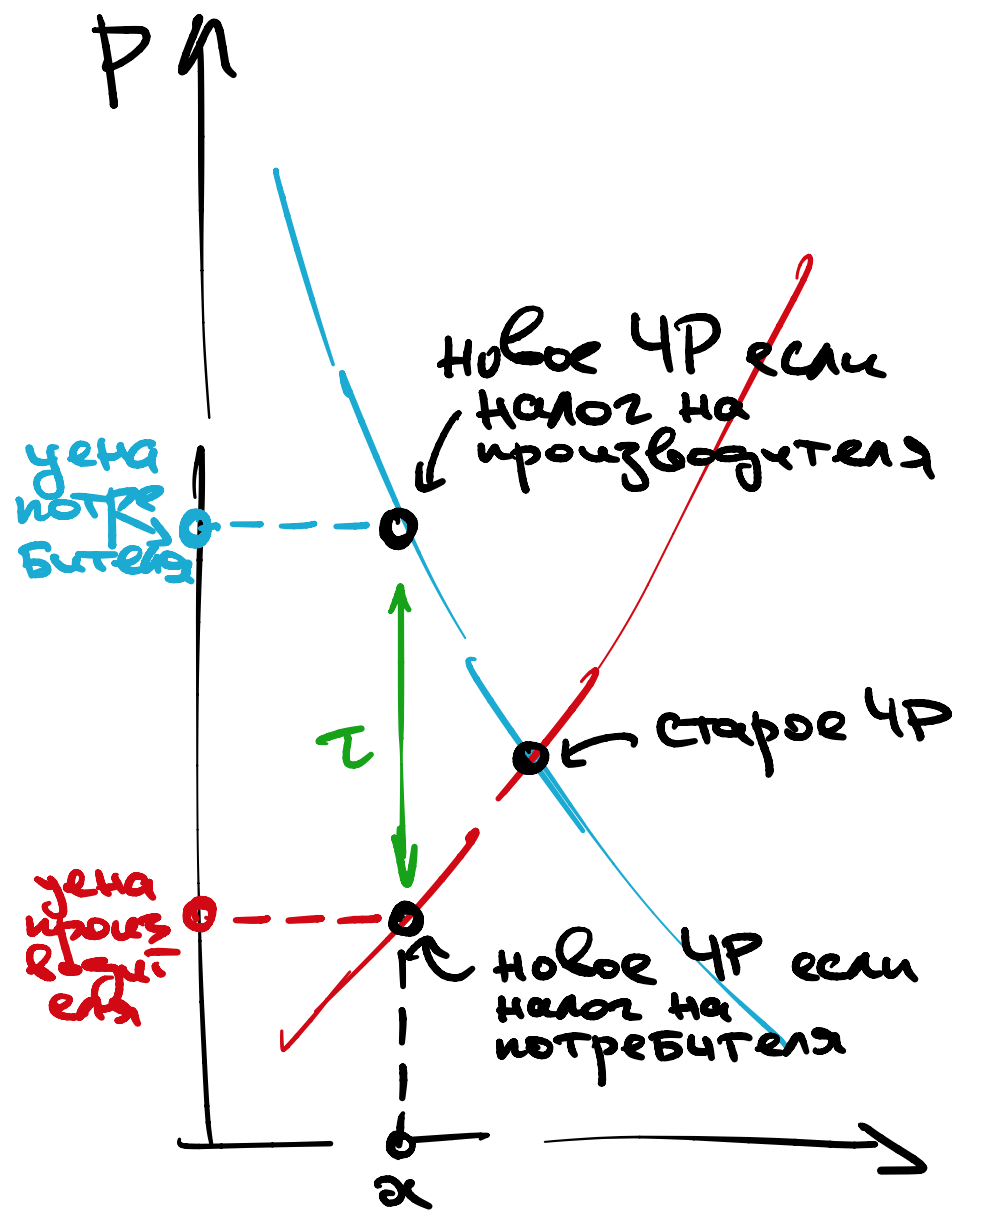
\includegraphics[width=1\textwidth]{bothtax}
     \end{center}
\end{column}
\end{columns}
\end{frame}

\section{Решим пример у доски}

\section{Налоги и DWL}

\begin{frame}{T и DWL}
\begin{columns}
\begin{column}{0.5\textwidth}
   Введем два новых объекта
   
   \medskip
   
   Первый объект это суммарные налоговые сборы.
   
   \medskip
   
   Второй объект это суммарные потери общества, традиционно обозначаются $DWL$.
   
   \medskip
   
   Заметим, что налог распределяется между агентами независимо от того, кто его платит номинально.
   
\end{column}
\begin{column}{0.5\textwidth}  %%<--- here
    \begin{center}
     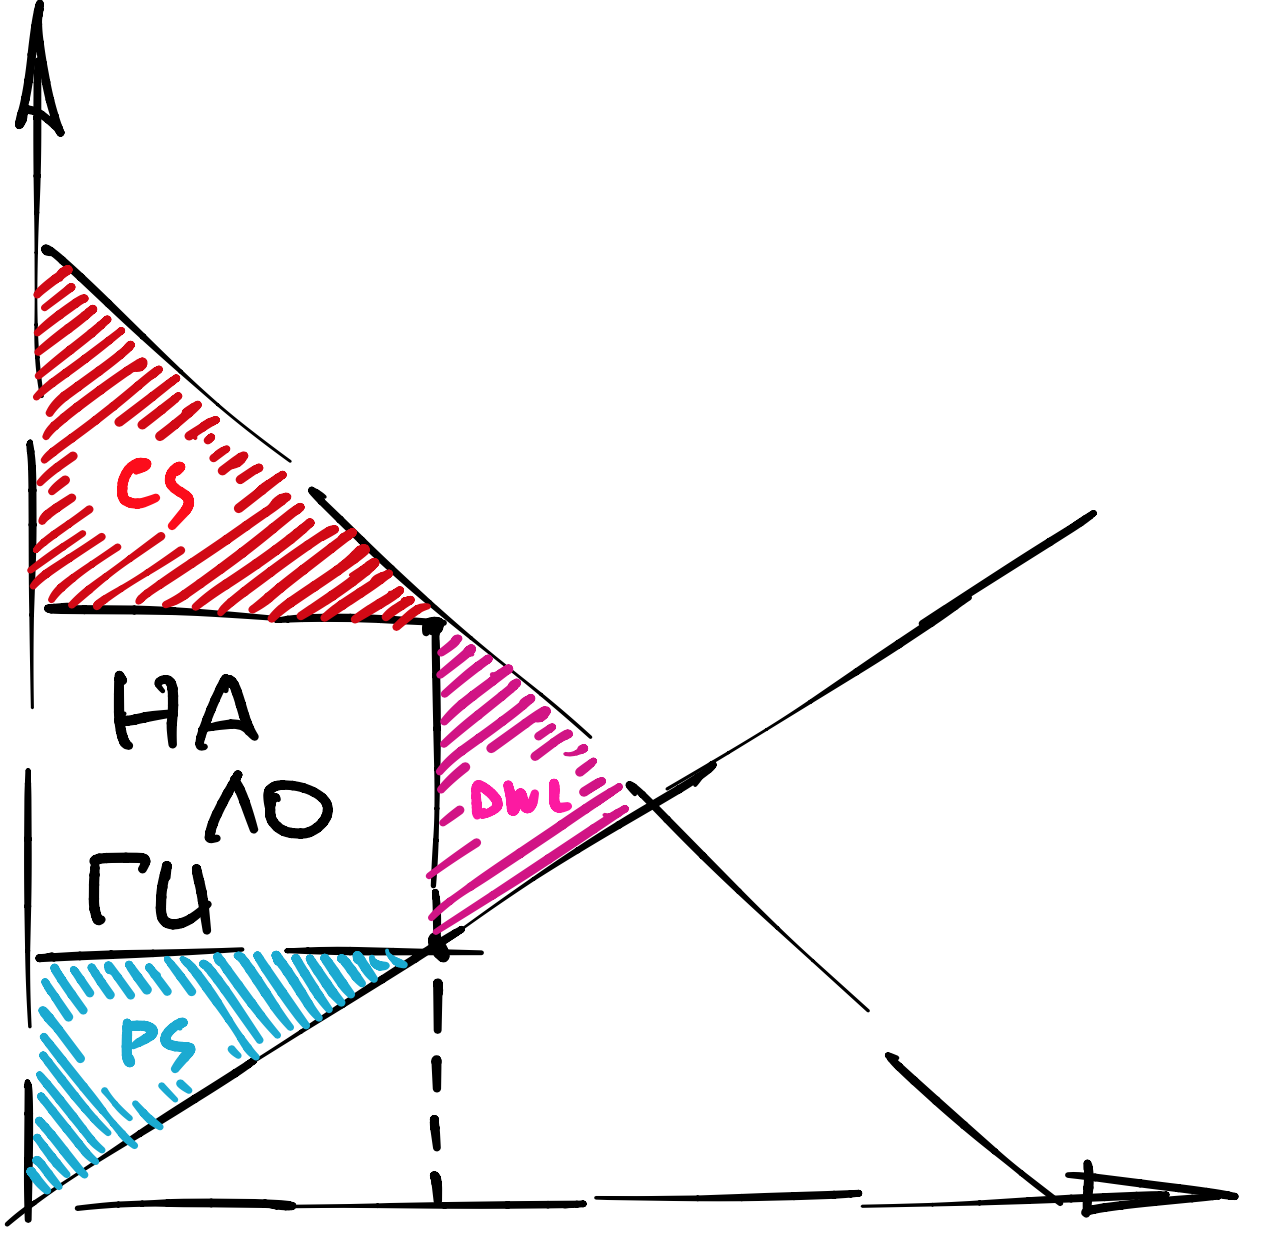
\includegraphics[width=1\textwidth]{taxesDWL}
     \end{center}
\end{column}
\end{columns}
\end{frame}

\begin{frame}{T и DWL}
\begin{columns}
\begin{column}{0.5\textwidth}
   Найдем налог в процентах от товарооборота $p x$ в равно-сии, причем \alert{приближенно}.
   
   \medskip
   Доля потребителя это $$\frac{\Delta^c p (x - \Delta x)}{px} = \frac{1}{|\varepsilon|}\frac{\Delta x}{x} (1 - \frac{\Delta x}{x})$$
    
   \medskip
   Доля производителя это $$\frac{\Delta^p p (x - \Delta x)}{px} = \frac{1}{|\mathcal{E}|}\frac{\Delta x}{x} (1 - \frac{\Delta x}{x})$$
   
   \medskip
   То есть, \alert{налог распределяется обратно пропорционально эластичностям} $\varepsilon$ и $\mathcal{E}$.
\end{column}
\begin{column}{0.5\textwidth}  %%<--- here
    \begin{center}
     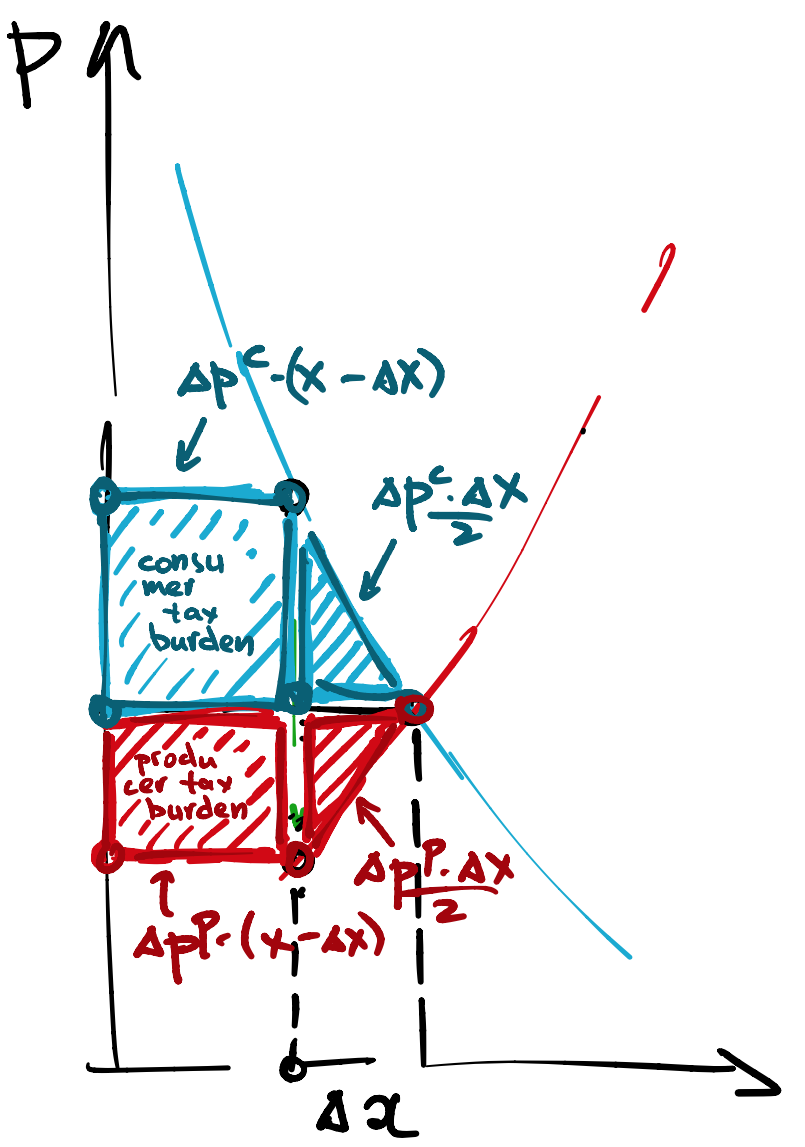
\includegraphics[width=1\textwidth]{taxburden}
     \end{center}
\end{column}
\end{columns}
\end{frame}

\begin{frame}{Налог в ЧР}

Похожим образом, я могу сосчитать DWL приближенно, и \alert{в процентах от товарооборота}, если мои входные данные это эластичность спроса $\varepsilon$, эластичность предложения $\mathcal{E}$ и налог, который задан в процентах от цены, естественно.
$$ \frac{DWL}{px} = \frac{\Delta p \Delta x}{2 p x} = \frac{1}{2}(\frac{\Delta p}{p})^2  \frac{p}{\Delta^p p + \Delta^c p} \frac{\Delta x}{x} = \frac{1}{2}\frac{1}{\frac{1}{|\varepsilon|} + \frac{1}{|\mathcal{E}|}} (\frac{\Delta p}{p})^2$$
То есть, DWL монотонно растет по эластичностям спросов. 

Чем менее эластичны спрос и предложение, тем меньше, в каком то смысле, страдает общество.

\end{frame}

\section{Субсидии}

\begin{frame}{Субсидии}
\begin{columns}
\begin{column}{0.4\textwidth}
   Когда субсидия, ситуация сложнее.
   
   \medskip
   \alert{Расщепление цен происходит так, что цена потребителя ниже чем цена производителя, однако налоговые сборы отрицательны}.
   
   \medskip
   PS, CS, T получаются с нахлестом, но если аккуратно сосчитать площади то можно снова найти DWL (он справа).
\end{column}
\begin{column}{0.6\textwidth}  %%<--- here
    \begin{center}
     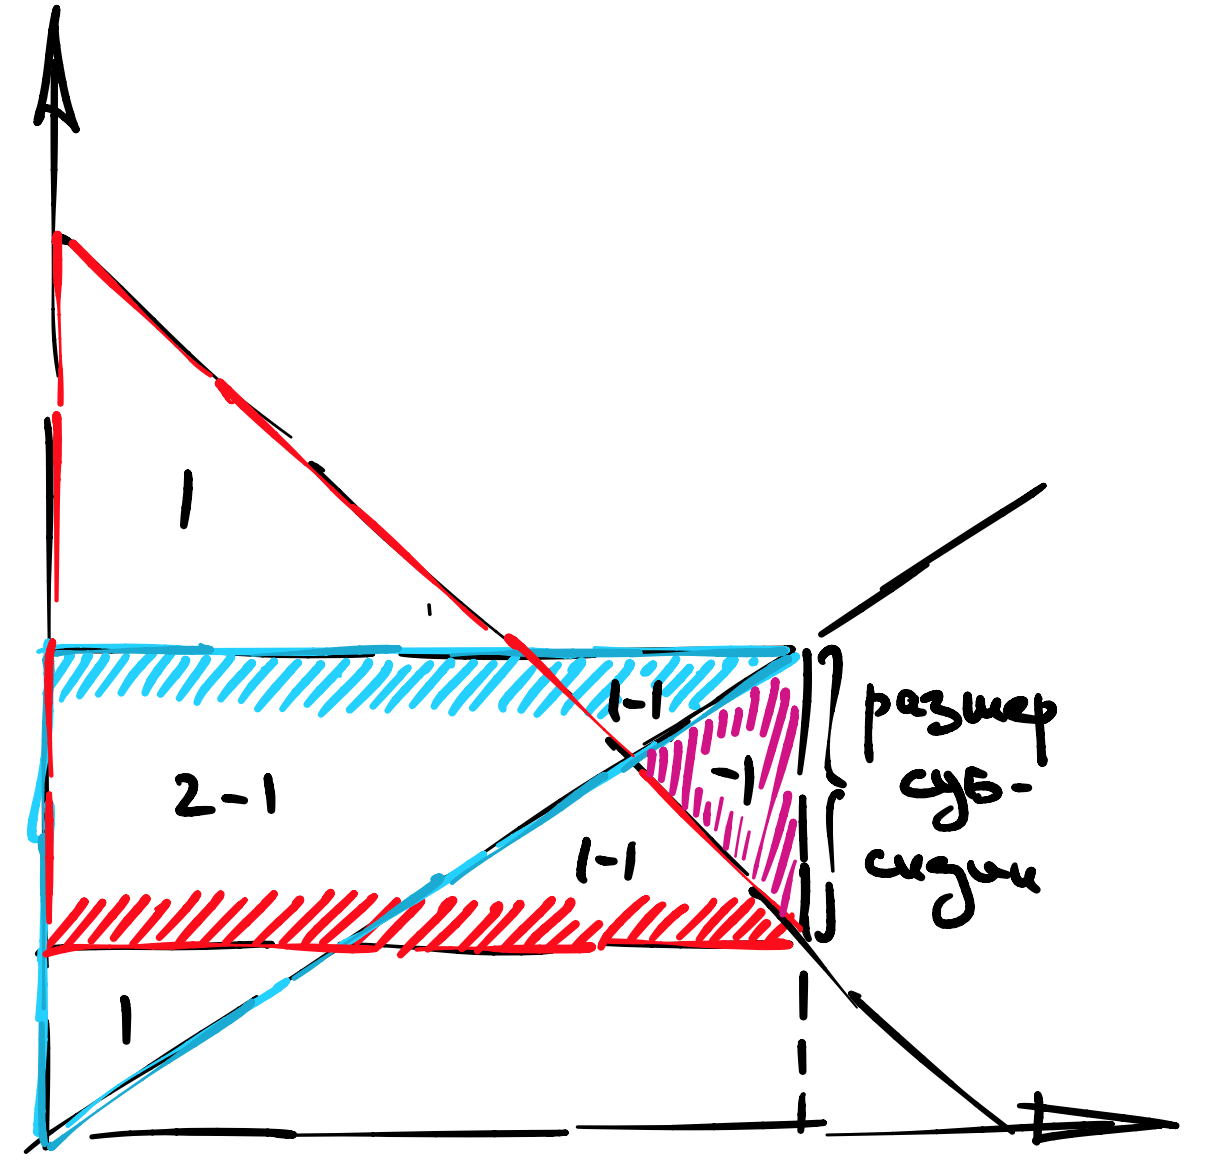
\includegraphics[width=1\textwidth]{subsidy}
     \end{center}
\end{column}
\end{columns}
\end{frame}

\section{Пол, потолок и экстерналии (на доске)}

\end{document}